\chapter{Contexte général et étude du projet}

\section{Introduction}
Ce premier chapitre situe le projet dans son contexte. Nous rappelons d'abord les notions essentielles de
l'Internet des objets et la manière dont l'intelligence artificielle l'enrichit. Nous présentons ensuite le projet,
la problématique qu'il traite et les objectifs fixés. Nous terminons par le cahier des charges, formalisé par un
diagramme de cas d'utilisation, et par l'architecture générale du système.

% ------------------------------------------------------------------------------------------------
\section{Généralités sur l'Internet des Objets (IoT)}

L'Internet des objets désigne l'extension d'Internet à des objets physiques dotés de capteurs, d'actionneurs, d'une
capacité de calcul et d'une interface de communication. Ces objets collectent des données sur leur
environnement, les transmettent à des services distants qui les analysent, et peuvent recevoir en retour des
commandes~\cite{atzori2010,alfuqaha2015}. La valeur d'un système IoT ne vient pas d'un objet isolé, mais de la
chaîne complète qui transforme une mesure brute en information utile, puis en décision.

\subsection*{Architecture en couches}
On décrit classiquement un système IoT par une architecture en couches (figure~\ref{fig:couches-iot}) :
\begin{itemize}
  \item la \textbf{couche perception}, formée des capteurs et des actionneurs (dans notre cas : capteurs
        infrarouges, capteur ultrasonique, caméra, moteurs) ;
  \item la \textbf{couche réseau}, qui achemine les données (Wi-Fi, Bluetooth, réseaux cellulaires, LoRa…) avec des
        protocoles applicatifs comme HTTP ou MQTT ;
  \item la \textbf{couche traitement}, qui stocke et analyse les données sur un serveur, dans le nuage ou en
        périphérie de réseau (\textit{edge}) ;
  \item la \textbf{couche application}, qui présente l'information à l'utilisateur et lui permet d'agir.
\end{itemize}

\begin{figure}[H]
\centering
\begin{tikzpicture}[couche/.style={draw=#1,very thick,fill=#1!12,rounded corners=4pt,minimum width=8.4cm,
                    text width=8cm,minimum height=1.15cm,align=left,font=\small},
                    projet/.style={draw=#1,thick,fill=white,rounded corners=4pt,minimum width=4.6cm,text width=4.3cm,
                    minimum height=1.15cm,align=center,font=\small\itshape}]
  \foreach \y/\c/\n/\t/\p in {4.5/bleufst/app/{\textbf{Application} — tableaux de bord, cartes, alertes, aide à la décision}/{SmartCar Ops (Dash)},
                             3/vertfst!80!black/tr/{\textbf{Traitement} — stockage, analyse, intelligence artificielle}/{SQLite, YOLO26, ONNX Runtime},
                             1.5/orangefst/res/{\textbf{Réseau} — transport des données et protocoles}/{Wi-Fi, HTTP / MJPEG},
                             0/gris/per/{\textbf{Perception} — capteurs et actionneurs}/{IR, HC-SR04, ESP32-CAM, moteurs}}
    {\node[couche=\c] (\n) at (-1.9,\y) {\t};
     \node[projet=\c] (\n p) at (5.0,\y) {\p};
     \draw[gris,dashed] (\n.east) -- (\n p.west);}
  \foreach \a/\b in {per/res,res/tr,tr/app} \draw[fleche,draw=gris] ([xshift=-0.35cm]\a.north west) -- ([xshift=-0.35cm]\b.south west);
  \foreach \a/\b in {app/tr,tr/res,res/per} \draw[fleche,draw=gris] ([xshift=0.35cm]\a p.south east) -- ([xshift=0.35cm]\b p.north east);
  \node[note,rotate=90] at (-6.75,2.25) {données};
  \node[note,rotate=90] at (8.05,2.25) {commandes};
  \node[font=\scriptsize\bfseries,gris] at (-1.9,5.4) {Couches de l'IoT};
  \node[font=\scriptsize\bfseries,gris] at (5.0,5.4) {Dans notre projet};
\end{tikzpicture}
\caption{Architecture en couches d'un système IoT et correspondance avec notre projet}
\label{fig:couches-iot}
\end{figure}

\subsection*{Domaines d'application et enjeux}
L'IoT est présent dans la maison connectée, l'industrie (maintenance prédictive), l'agriculture de précision, la
santé et, bien sûr, le transport : véhicules connectés, gestion du trafic, surveillance de l'état des routes. Ce
déploiement massif soulève plusieurs enjeux : les contraintes énergétiques des objets, la fiabilité des
communications sans fil, le volume des données à traiter, la sécurité et la confidentialité, et l'interopérabilité
entre équipements hétérogènes~\cite{gubbi2013}.

% ------------------------------------------------------------------------------------------------
\section{IoT et Intelligence Artificielle}

Les objets connectés produisent des données en grande quantité, mais ces données n'ont de valeur que si elles sont
interprétées. L'association de l'IoT et de l'intelligence artificielle, parfois appelée \emph{AIoT}
(\textit{Artificial Intelligence of Things}), consiste à confier cette interprétation à des modèles
d'apprentissage automatique~\cite{zhang2021aiot}. Une caméra connectée ne transmet alors plus seulement des
images : elle permet de savoir \emph{quels} objets se trouvent devant le véhicule, \emph{où} ils se trouvent et
\emph{à quel point} ils sont dangereux.

Deux stratégies de déploiement coexistent :
\begin{itemize}
  \item l'\textbf{inférence en périphérie} (\textit{edge AI}), sur l'objet lui-même ou à proximité, qui réduit la
        latence et la bande passante mais est limitée par la puissance de calcul et l'énergie disponibles ;
  \item l'\textbf{inférence sur serveur ou dans le nuage}, qui permet d'utiliser des modèles plus lourds au prix
        d'une dépendance au réseau.
\end{itemize}
Dans notre projet, la caméra ESP32-CAM ne dispose ni de la mémoire ni de la puissance nécessaires pour exécuter un
détecteur moderne à une cadence utile. Elle se contente donc d'acquérir et de diffuser les images en Wi-Fi ;
l'inférence est réalisée sur un serveur local (l'ordinateur portable qui héberge l'application), au plus près du
véhicule. Les modèles ont été choisis légers (variantes \emph{nano} et \emph{small} de YOLO26) et exportés au
format ONNX afin de rester exécutables en temps réel sur processeur, ce qui préserve la possibilité d'un
déploiement embarqué ultérieur.

% ------------------------------------------------------------------------------------------------
\section{Présentation du projet}

Le projet consiste à concevoir un système intelligent qui détecte les obstacles présents sur le trajet d'un
véhicule, en évalue la gravité et met ces informations à disposition d'un opérateur à travers une application de
supervision. Il est composé de trois éléments (figure~\ref{fig:projet}) :
\begin{enumerate}
  \item \textbf{Le prototype} : une voiture miniature qui suit une piste tracée au ruban adhésif noir grâce à deux
        capteurs infrarouges, mesure la distance qui la sépare d'un obstacle avec un capteur ultrasonique, et
        embarque une caméra ESP32-CAM qui filme la route de son point de vue.
  \item \textbf{Les modèles d'intelligence artificielle} : des détecteurs d'objets YOLO26 qui reconnaissent les
        obstacles dans les images, d'une part sur des routes réelles, d'autre part sur la piste du prototype.
  \item \textbf{L'application \app} : un tableau de bord web qui exécute les modèles, localise et priorise les
        obstacles, suit les véhicules, planifie des itinéraires et présente des statistiques.
\end{enumerate}

L'application fonctionne dans \textbf{deux environnements}, sélectionnés par un commutateur dans la barre
supérieure :
\begin{itemize}
  \item \textbf{Monde réel} : une flotte de trois véhicules simulés circule sur le réseau routier réel du Quartier
        Latin à Paris (données OpenStreetMap). Le véhicule CAR-01 est équipé d'une « caméra embarquée » virtuelle
        qui lit de vraies vidéos de route ; nos modèles les analysent en temps réel et les obstacles détectés sont
        placés sur la carte devant le véhicule.
  \item \textbf{Prototype} : la voiture miniature sur sa piste. Les informations proviennent uniquement de
        l'image de l'ESP32-CAM (obstacles détectés, marqueurs de points de passage, mouvement), car la carte
        Arduino n'a pas de liaison sans fil.
\end{itemize}

\begin{figure}[H]
\centering
\begin{subfigure}[b]{0.40\linewidth}\centering
  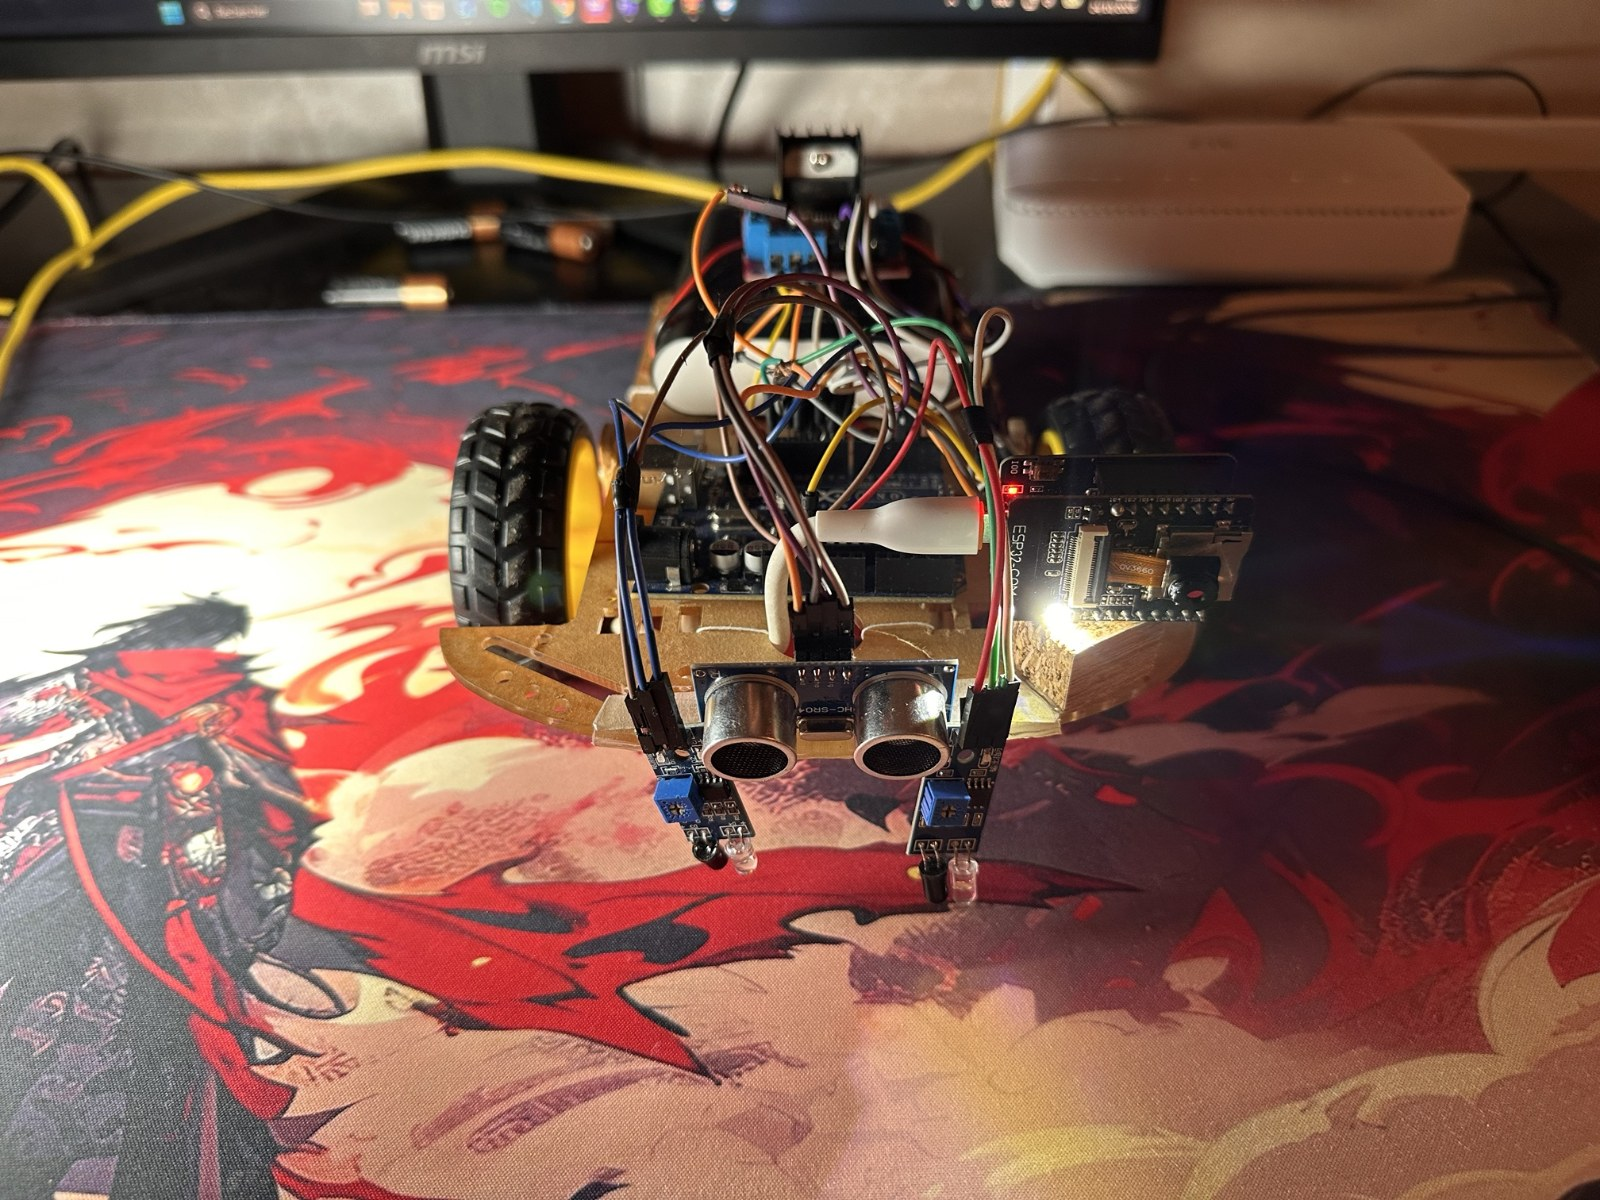
\includegraphics[height=4.6cm]{photos/prototype_avant.jpg}
  \caption{Le prototype}
\end{subfigure}\hfill
\begin{subfigure}[b]{0.31\linewidth}\centering
  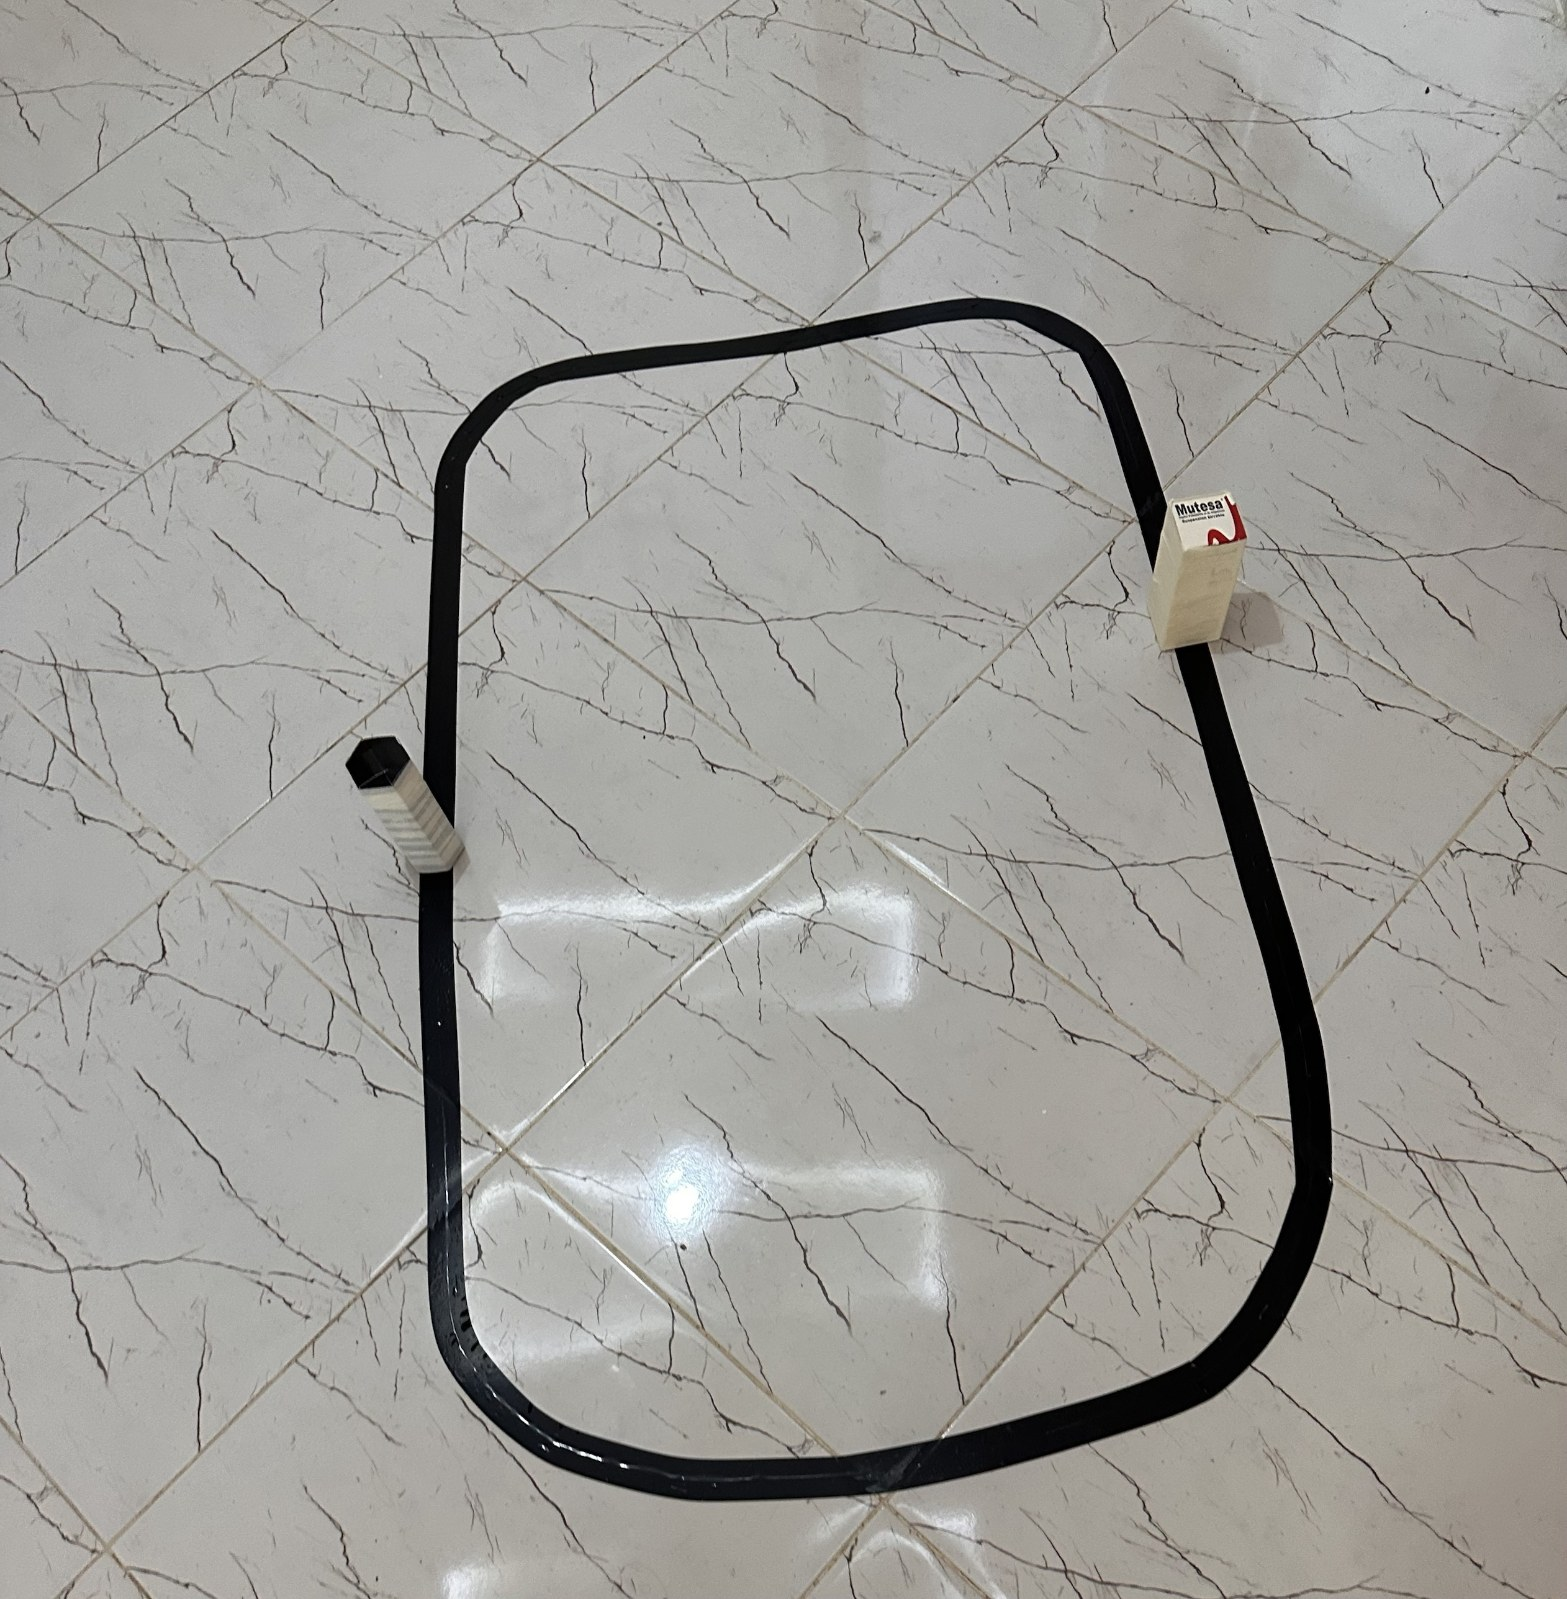
\includegraphics[height=4.6cm]{photos/piste.jpg}
  \caption{La piste et ses obstacles}
\end{subfigure}\hfill
\begin{subfigure}[b]{0.24\linewidth}\centering
  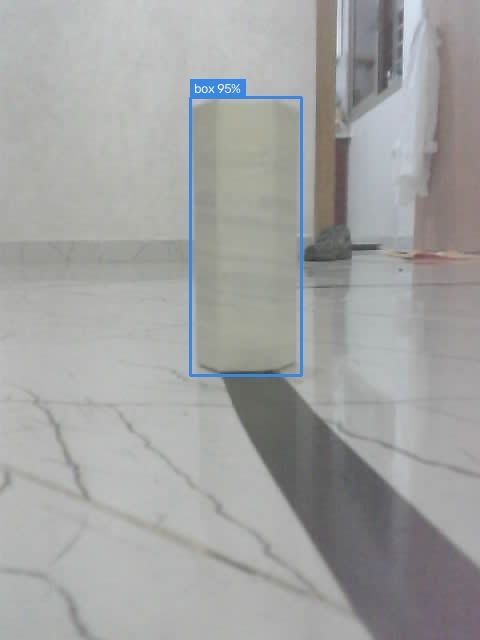
\includegraphics[height=4.6cm]{captures/esp32_detection_box.jpg}
  \caption{Vue de la caméra et détection}
\end{subfigure}

\vspace{0.3cm}
\begin{subfigure}[b]{0.49\linewidth}\centering
  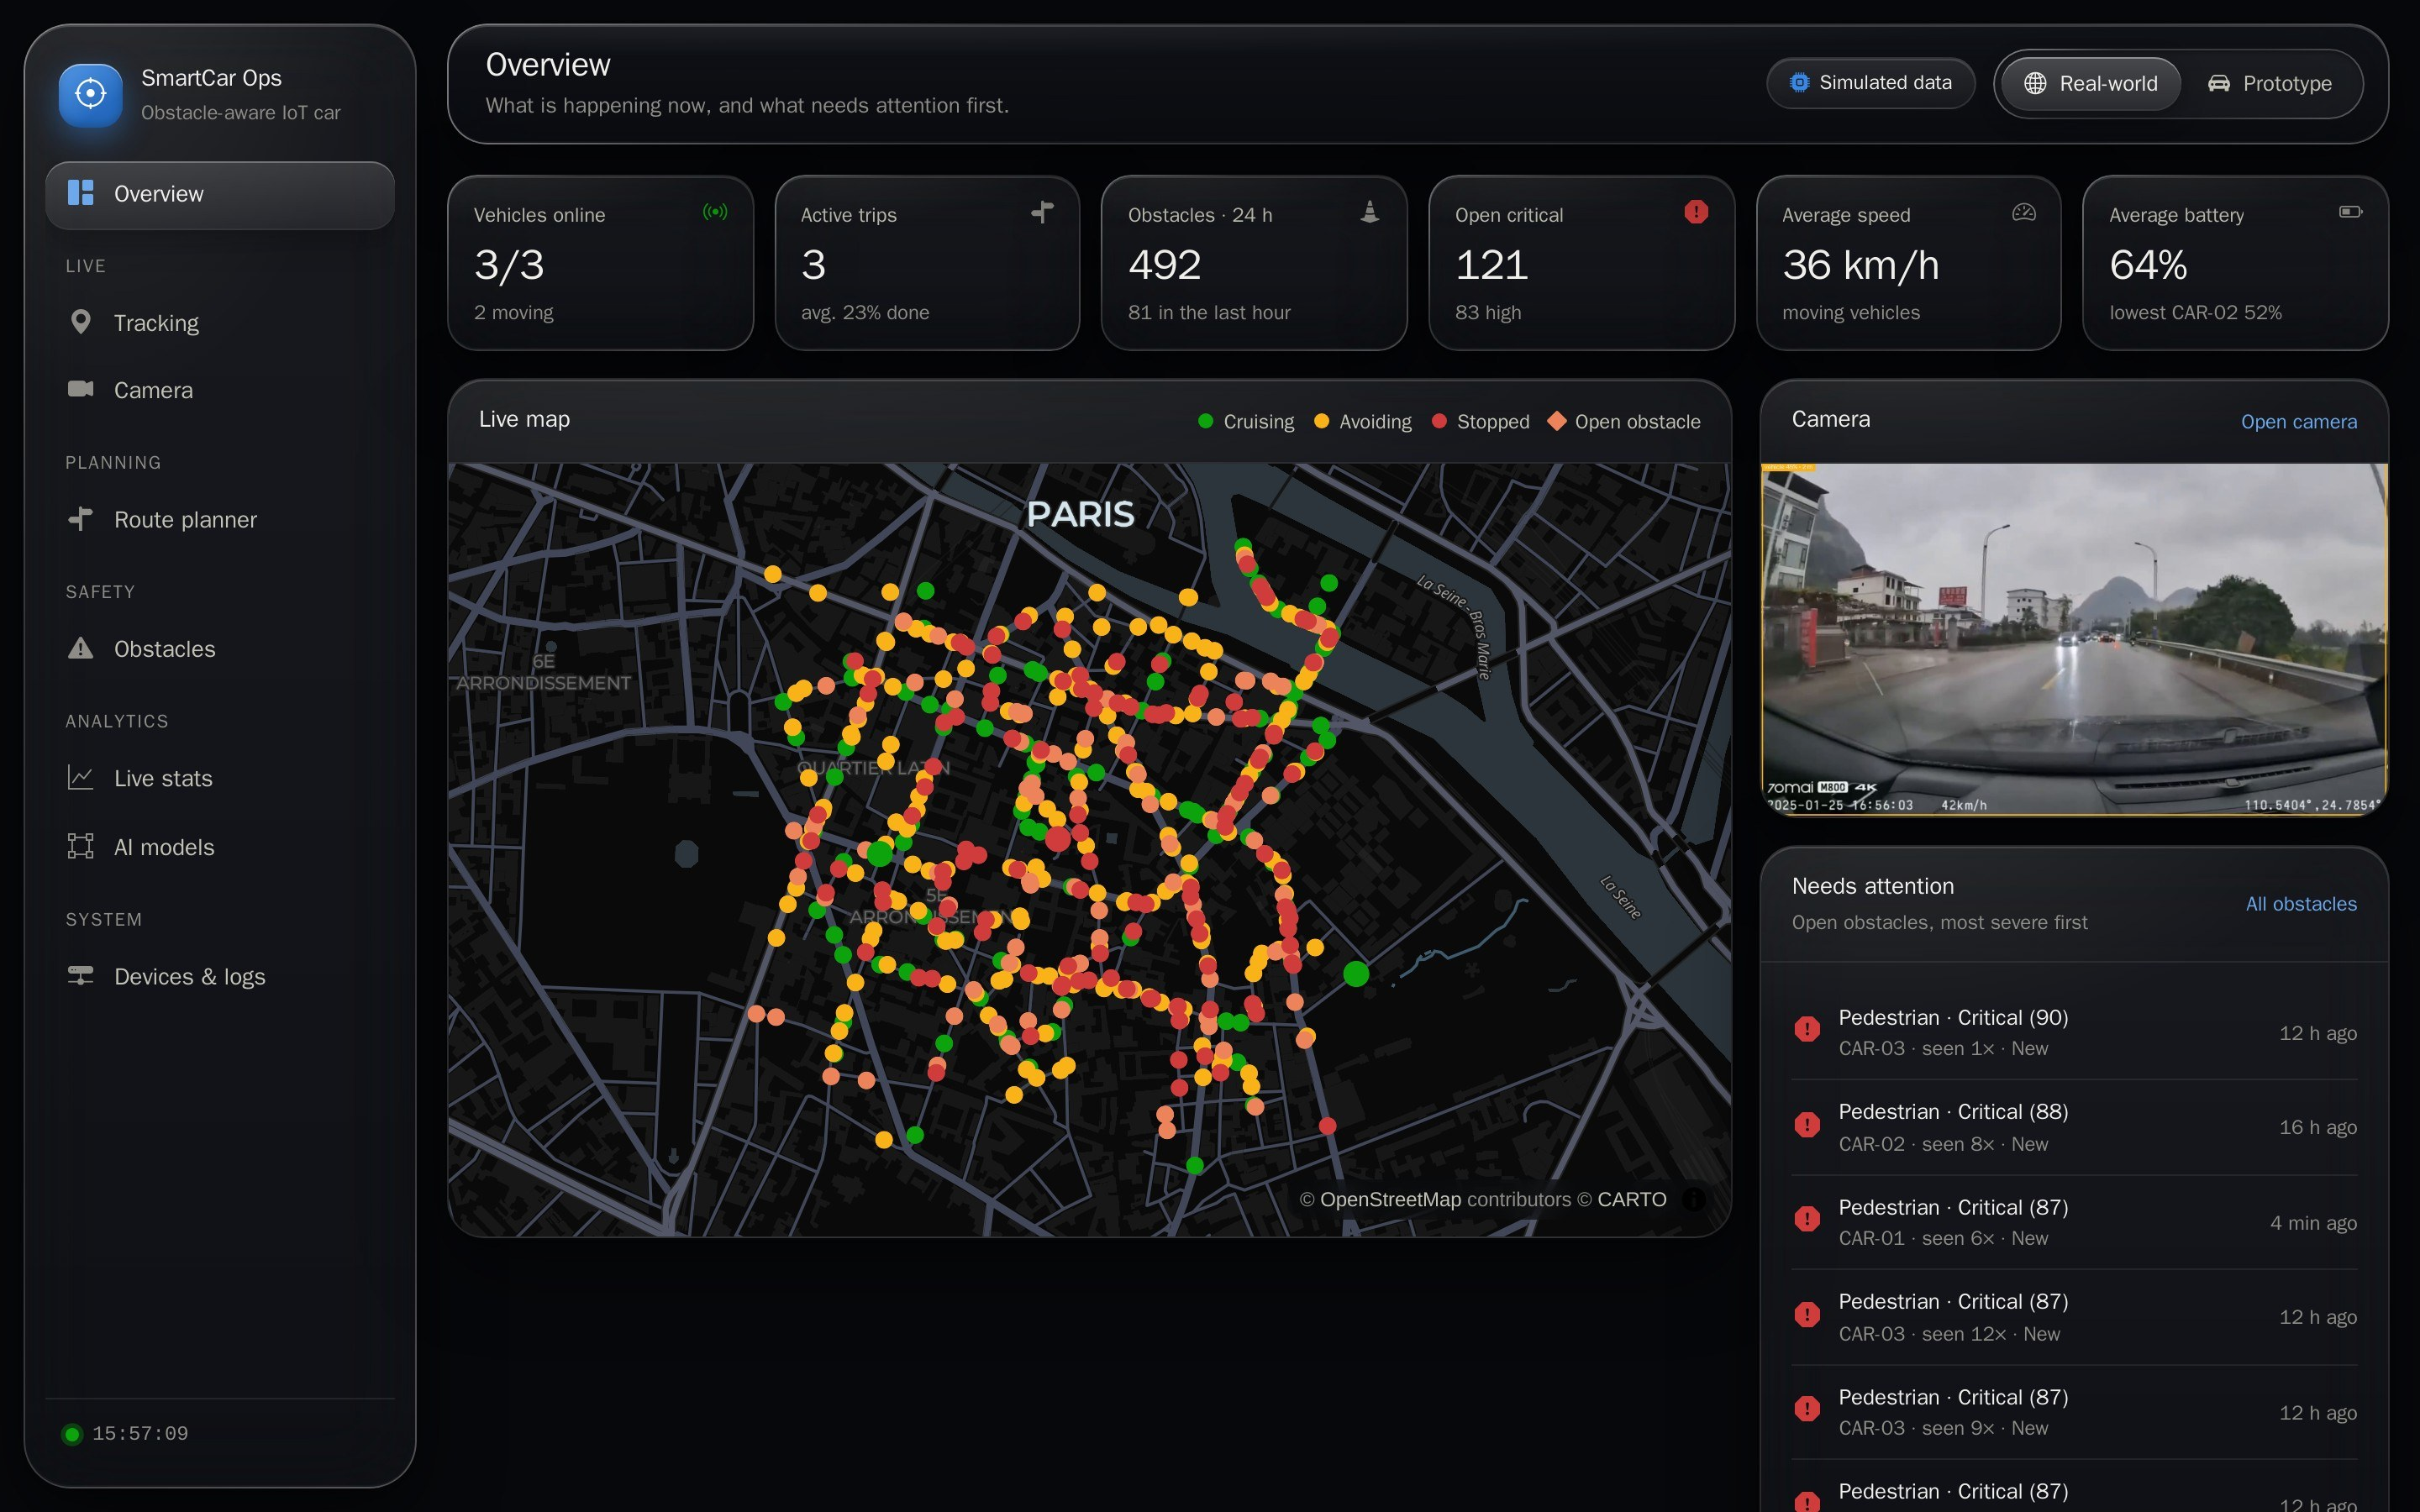
\includegraphics[width=\linewidth]{captures/overview_real_ecran.jpg}
  \caption{Environnement \emph{Monde réel}}
\end{subfigure}\hfill
\begin{subfigure}[b]{0.49\linewidth}\centering
  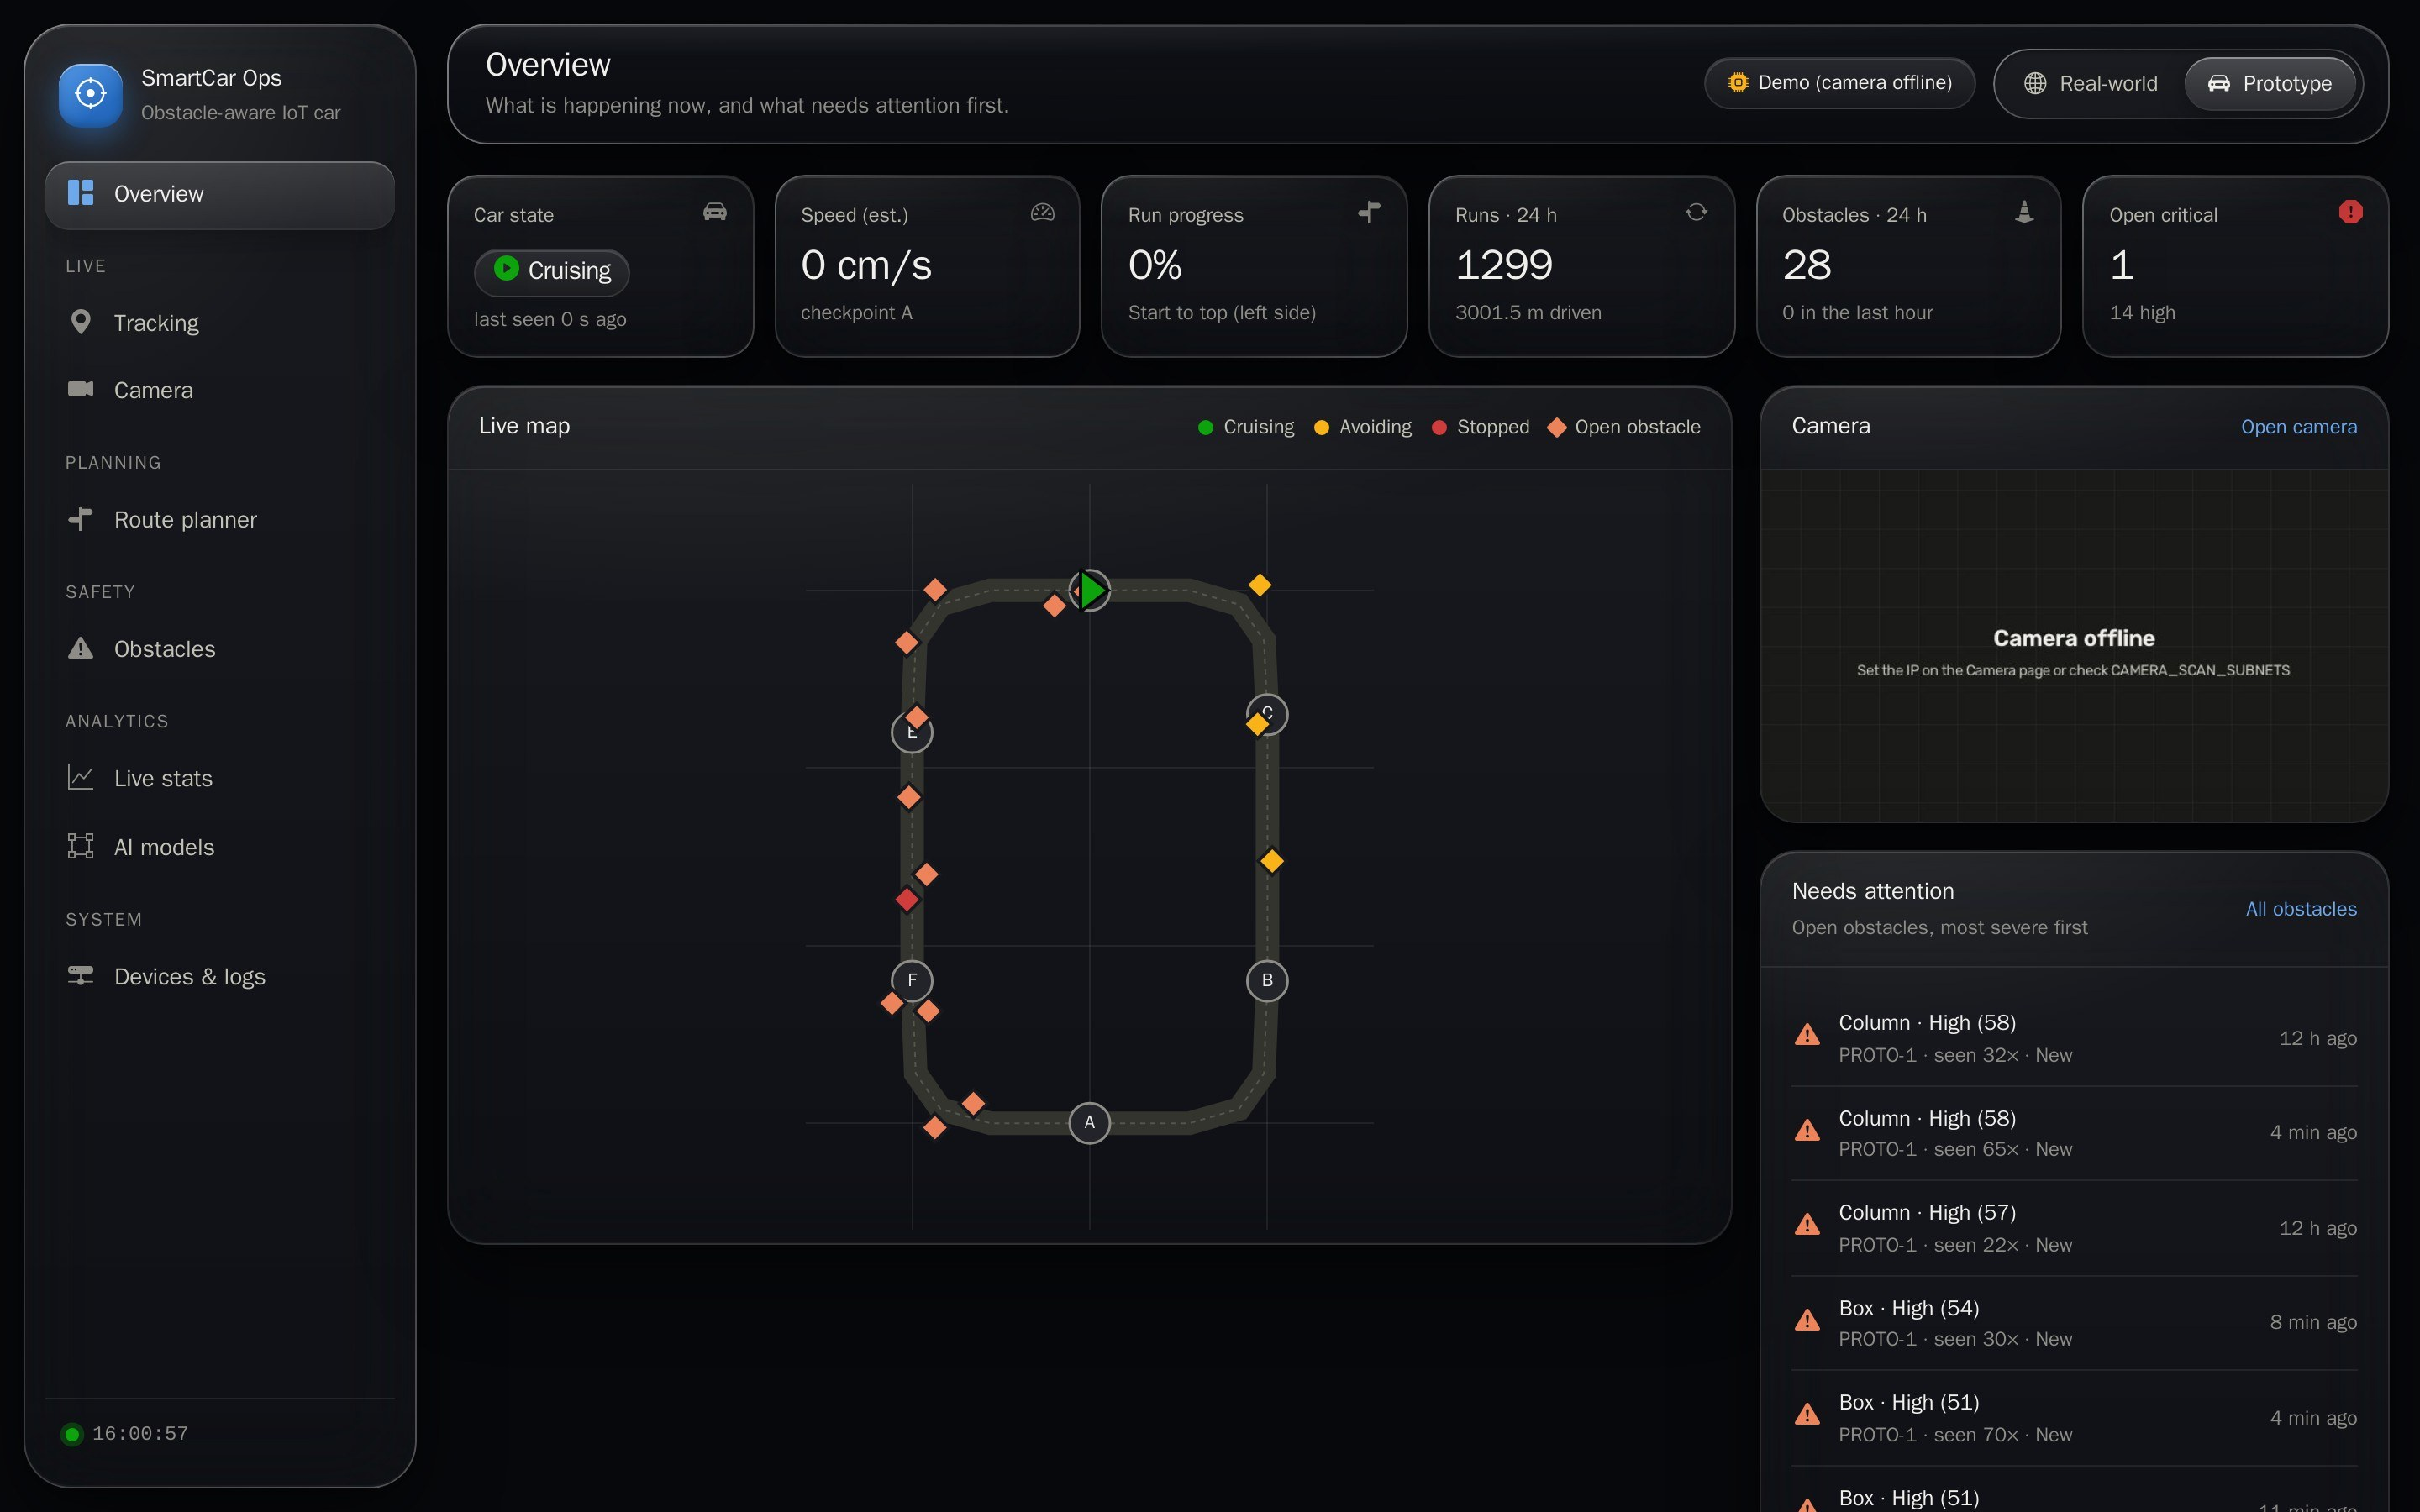
\includegraphics[width=\linewidth]{captures/overview_proto_ecran.jpg}
  \caption{Environnement \emph{Prototype}}
\end{subfigure}
\caption{Le prototype, l'application \app{} et ses deux environnements}
\label{fig:projet}
\end{figure}

% ------------------------------------------------------------------------------------------------
\section{Problématique}

La détection des obstacles routiers pose plusieurs difficultés. Les obstacles sont très variés : usagers mobiles
(piétons, cyclistes, véhicules, animaux) et anomalies statiques (nids-de-poule, cônes, barrières, panneaux de
chantier). Ils apparaissent dans des conditions changeantes de lumière, de météo et de point de vue. Les
nids-de-poule, en particulier, sont plats, de forme irrégulière et souvent peu contrastés.

Détecter ne suffit pas : un opérateur a besoin de savoir \emph{où} se trouve l'obstacle, \emph{à quel point} il
est dangereux et \emph{lequel traiter en premier}. Ces informations doivent ensuite servir à la décision, par
exemple au choix d'un itinéraire. Enfin, le prototype impose ses propres contraintes : une carte Arduino aux
ressources très limitées, une caméra peu coûteuse dont l'adresse IP change à chaque connexion, et aucune liaison
de communication entre l'Arduino et la caméra.

La problématique du projet peut donc se formuler ainsi :
\begin{center}
\begin{minipage}{0.9\linewidth}\itshape
Comment concevoir, avec des composants à faible coût, un système IoT capable de détecter automatiquement les
obstacles sur le trajet d'un véhicule, d'en évaluer la gravité et la priorité, et d'exploiter ces informations
en temps réel pour la supervision et la planification d'itinéraires, aussi bien sur des routes réelles que sur un
prototype à échelle réduite ?
\end{minipage}
\end{center}

% ------------------------------------------------------------------------------------------------
\section{Objectifs du projet}

Les objectifs fixés sont les suivants :
\begin{enumerate}
  \item \textbf{Réaliser le prototype} : assembler et câbler une voiture miniature capable de suivre une piste et
        de réagir à un obstacle, équipée d'une caméra Wi-Fi.
  \item \textbf{Entraîner des modèles de détection} : choisir des jeux de données réels d'obstacles routiers,
        entraîner un détecteur dans un environnement reproductible (notebook Jupyter dans un conteneur Docker), puis
        constituer et annoter un jeu de données propre à notre piste pour entraîner le modèle du prototype.
  \item \textbf{Évaluer honnêtement les modèles} : mesurer la précision, le rappel, le score F1, le mAP et le
        temps d'inférence sur des données jamais vues pendant l'entraînement.
  \item \textbf{Exploiter les détections} : estimer la distance et la gravité des obstacles, leur attribuer une
        priorité, les localiser et les fusionner lorsqu'ils sont vus plusieurs fois.
  \item \textbf{Développer l'application \app} : suivi des véhicules, flux vidéo annoté, planification
        d'itinéraires tenant compte des obstacles, gestion des anomalies, statistiques, présentation des modèles,
        surveillance des périphériques et des journaux, pour les deux environnements.
  \item \textbf{Assurer un déploiement simple} : l'ensemble du logiciel doit se lancer avec Docker, sans
        installation manuelle de bibliothèques.
\end{enumerate}

% ------------------------------------------------------------------------------------------------
\section{Cahier des charges}

\subsection*{Besoins fonctionnels}
\begin{itemize}
  \item \textbf{BF1 — Deux environnements} : basculer à tout moment entre \emph{Monde réel} et \emph{Prototype} ;
        chaque page s'adapte (unités en mètres ou en centimètres, carte routière ou plan de la piste).
  \item \textbf{BF2 — Vue d'ensemble} : indicateurs clés, carte en direct, obstacles à traiter, derniers
        événements.
  \item \textbf{BF3 — Suivi} : position des véhicules en temps réel, traces, état, historique des trajets et
        relecture d'un trajet passé.
  \item \textbf{BF4 — Caméra} : afficher le flux de l'ESP32-CAM malgré une adresse IP dynamique (découverte
        automatique), ou les vidéos de la caméra embarquée, avec les détections superposées.
  \item \textbf{BF5 — Planification} : choisir un départ et une destination, proposer l'itinéraire le plus court,
        le plus sûr et un compromis réglable ; éditer la piste du prototype et ses trajectoires.
  \item \textbf{BF6 — Obstacles} : liste triée par priorité, filtres, détail avec instantané, carte, actions
        (acquitter, résoudre, marquer comme faux positif).
  \item \textbf{BF7 — Statistiques} : répartitions par classe, par gravité, par heure, états des véhicules.
  \item \textbf{BF8 — Modèles d'IA} : métriques d'évaluation, matrice de confusion, comportement sur la route.
  \item \textbf{BF9 — Périphériques et journaux} : état des équipements, journal des événements, réglages
        (poids de danger des classes, données de démonstration).
\end{itemize}

\subsection*{Besoins non fonctionnels}
\begin{itemize}
  \item \textbf{Temps réel} : rafraîchissement des données chaque seconde ; analyse vidéo sur processeur sans
        bloquer l'affichage (seule l'image la plus récente est analysée).
  \item \textbf{Fiabilité} : reconnexion automatique de la caméra, base de données robuste (SQLite en mode WAL dans
        un volume Docker).
  \item \textbf{Ergonomie} : interface claire et cohérente, couleurs de gravité toujours accompagnées d'une icône et
        d'un libellé.
  \item \textbf{Portabilité et reproductibilité} : application et entraînement conteneurisés (Docker).
  \item \textbf{Évolutivité} : détecteur interchangeable (profils de modèles ONNX), configuration par variables
        d'environnement.
  \item \textbf{Honnêteté des mesures} : métriques calculées sur des ensembles de test séparés, avec le réglage
        utilisé clairement indiqué.
\end{itemize}

\subsection*{Diagramme de cas d'utilisation}
Le diagramme de la figure~\ref{fig:usecase} résume les interactions entre les acteurs et le système. L'opérateur
supervise les véhicules et les obstacles ; l'administrateur, qui est un opérateur avec des droits de
configuration, règle la caméra, la piste et les poids de danger. La caméra ESP32-CAM et la caméra embarquée du
monde réel sont des acteurs secondaires qui fournissent les images.

\begin{figure}[H]
\centering
\resizebox{\linewidth}{!}{%
\begin{tikzpicture}[
  uc/.style={ellipse,draw=bleufst,thick,fill=bleufst!7,minimum width=5.0cm,minimum height=1.05cm,align=center,
             font=\footnotesize,inner sep=0pt},
  ucs/.style={uc,draw=orangefst,fill=orangefst!10},
  lien/.style={thick,draw=encre!80},
  inc/.style={-{Stealth[length=2mm]},dashed,draw=gris,thick},
  st/.style={font=\scriptsize\itshape,text=gris,fill=white,inner sep=1pt},
  pics/acteur/.style={code={
     \draw[very thick,encre] (0,0.62) circle (0.2);
     \draw[very thick,encre] (0,0.42) -- (0,-0.12) (-0.34,0.24) -- (0.34,0.24) (0,-0.12) -- (-0.26,-0.6)
                             (0,-0.12) -- (0.26,-0.6);}}]
  % frontière du système
  \draw[thick,rounded corners=6pt,fill=fond] (-5.6,-7.3) rectangle (5.9,7.6);
  \node[font=\bfseries] at (0.15,7.2) {Système \app};
  % cas d'utilisation de l'opérateur
  \foreach \i/\t in {1/{Changer d'environnement\\(Monde réel / Prototype)},2/Consulter la vue d'ensemble,
                     3/{Suivre les véhicules\\et rejouer un trajet},4/{Visualiser le flux vidéo\\et les détections},
                     5/Planifier un itinéraire,6/{Gérer les obstacles (acquitter,\\résoudre, faux positif)},
                     7/Consulter les statistiques,8/Consulter les modèles d'IA,
                     9/{Surveiller les périphériques\\et les journaux}}
     \node[uc] (u\i) at (-2.75,7.95-1.6*\i) {\t};
  % cas internes et cas de l'administrateur
  \node[ucs] (r1) at (3.1,5.8)  {Acquérir les images\\(flux MJPEG / vidéo)};
  \node[ucs] (r2) at (3.1,3.9)  {Détecter les obstacles\\(YOLO26)};
  \node[ucs] (r3) at (3.1,1.9)  {Estimer distance,\\gravité et priorité};
  \node[ucs] (r4) at (3.1,-0.1) {Calculer le risque\\des segments};
  \node[uc]  (a1) at (3.1,-2.6) {Configurer la caméra\\(IP, rotation, enregistrement)};
  \node[uc]  (a2) at (3.1,-4.3) {Éditer la piste\\et les trajectoires};
  \node[uc]  (a3) at (3.1,-6.0) {Régler les poids\\de danger des classes};
  % acteurs
  \pic at (-8.2,1.7) {acteur}; \node[font=\small\bfseries] (op) at (-8.2,0.75) {Opérateur};
  \coordinate (opc) at (-7.8,1.6);
  \pic at (8.6,-4.3) {acteur}; \node[font=\small\bfseries,align=center] (ad) at (8.6,-5.35) {Administrateur};
  \coordinate (adc) at (8.2,-4.2);
  \pic at (8.6,6.3) {acteur}; \node[font=\small\bfseries,align=center] at (8.6,5.25) {ESP32-CAM};
  \pic at (8.6,3.2) {acteur}; \node[font=\small\bfseries,align=center] at (8.6,2.05) {Caméra embarquée\\CAR-01 (vidéo)};
  % associations
  \foreach \i in {1,...,9} \draw[lien] (opc) -- (u\i.west);
  \foreach \a in {a1,a2,a3} \draw[lien] (adc) -- (\a.east);
  \draw[lien] (8.2,6.2) -- (r1.east);
  \draw[lien] (8.2,3.1) -- (r1.south east);
  % inclusions
  \draw[inc] (u4.east) -- node[st,pos=0.45] {«include»} (r2.west);
  \draw[inc] (r2.north) -- node[st] {«include»} (r1.south);
  \draw[inc] (r2.south) -- node[st] {«include»} (r3.north);
  \draw[inc] (u6.east) -- node[st,pos=0.4] {«include»} (r3.south west);
  \draw[inc] (u5.east) -- node[st,pos=0.5] {«include»} (r4.west);
  \draw[inc] (r4.north) -- node[st] {«include»} (r3.south);
  % généralisation administrateur -> opérateur
  \draw[thick,-{Triangle[open,length=3mm,width=3mm]}] (8.6,-6.0) -- (8.6,-8.0) -- (-8.2,-8.0) -- (-8.2,0.45);
\end{tikzpicture}}
\caption{Diagramme UML de cas d'utilisation de \app}
\label{fig:usecase}
\end{figure}

% ------------------------------------------------------------------------------------------------
\section{Architecture générale du système}

La figure~\ref{fig:architecture} présente l'architecture globale, organisée selon les couches de l'IoT.

\begin{itemize}
  \item \textbf{Perception.} Dans le prototype, l'Arduino UNO lit les deux capteurs infrarouges et le capteur
        ultrasonique, et pilote les deux moteurs à travers le L298N : c'est la boucle de commande embarquée, autonome.
        L'ESP32-CAM, alimentée séparément, filme la piste. Dans le monde réel, la perception est assurée par des
        vidéos de caméras embarquées et par un simulateur de flotte qui produit la télémétrie des véhicules.
  \item \textbf{Réseau.} L'ESP32-CAM diffuse un flux MJPEG en HTTP sur le réseau Wi-Fi local (port 81) et expose une
        interface de réglage (port 80). Son adresse IP étant attribuée dynamiquement, le serveur la retrouve par
        balayage du sous-réseau.
  \item \textbf{Traitement.} Un conteneur Docker héberge le serveur : relais du flux vidéo (la caméra n'accepte
        qu'un seul client), redressement de l'image, détection d'objets par les modèles YOLO26 exportés en ONNX,
        lecture des marqueurs ArUco, estimation de la distance, de la gravité et de la priorité, fusion des
        détections répétées, calcul du risque des segments et planification d'itinéraires. Les données sont
        stockées dans une base SQLite. Un second conteneur, utilisé hors ligne, sert à l'entraînement des modèles
        sur GPU (JupyterLab et Ultralytics).
  \item \textbf{Application.} L'application Dash présente les huit pages de supervision dans le navigateur de
        l'opérateur et se rafraîchit chaque seconde.
\end{itemize}

\begin{figure}[H]
\centering
\resizebox{\linewidth}{!}{%
% Architecture globale du système (figure du chapitre 1)
\begin{tikzpicture}[
  b/.style={bloc,font=\footnotesize,minimum width=3cm,text width=2.8cm,minimum height=1cm},
  bo/.style={b,draw=orangefst,fill=orangefst!12},
  bv/.style={b,draw=vertfst!80!black,fill=vertfst!15},
  bg/.style={b,fill=bleufst!10}]
  % ---- perception : prototype
  \node[bo] (sens) at (1.7,-0.75) {Capteurs IR\\+ HC-SR04};
  \node[bo] (uno)  at (1.7,-2.15) {Arduino UNO\\(commande)};
  \node[bo] (mot)  at (1.7,-3.55) {L298N\\+ 2 moteurs DC};
  \node[bo] (cam)  at (5.1,-2.15) {ESP32-CAM\\(OV3660)};
  \draw[fleche] (sens) -- (uno); \draw[fleche] (uno) -- (mot);
  \begin{scope}[on background layer]
    \node[zone,fill=orangefst!5,fit=(sens)(mot)(cam),
          label={[font=\bfseries\small]above:Prototype — perception}] (zp) {};
  \end{scope}
  % ---- perception : monde réel
  \node[bv] (vid) at (8.5,-2.15)  {Vidéos de route\\(dashcam de CAR-01)};
  \node[bv] (sim) at (12.0,-2.15) {Simulateur de flotte\\(3 véhicules)};
  \node[bv] (osm) at (15.5,-2.15) {Graphe routier OSM\\(Quartier Latin)};
  \begin{scope}[on background layer]
    \node[zone,fill=vertfst!6,fit=(vid)(osm)(vid|-sens.north)(vid|-mot.south),
          label={[font=\bfseries\small]above:Monde réel — perception}] (zr) {};
  \end{scope}
  % ---- réseau
  \node[b,draw=orangefst,fill=white] (wifi) at (5.1,-5.0) {Wi-Fi 802.11\\HTTP : flux MJPEG};
  \draw[fleche] (cam) -- (wifi);
  % ---- traitement (serveur)
  \node[bg] (relay) at (1.7,-7.2)  {Découverte IP\\+ relais MJPEG};
  \node[bg] (perc)  at (5.1,-7.2)  {Perception : rotation,\\ArUco, mouvement};
  \node[bg] (onnx)  at (8.5,-7.2)  {Inférence YOLO26\\(ONNX Runtime)};
  \node[bg] (sev)   at (13.2,-7.2) {Distance, gravité,\\priorité, fusion};
  \node[bg] (db)    at (5.1,-8.9)  {SQLite (WAL)\\+ instantanés};
  \node[bg] (hub)   at (8.5,-8.9)  {Télémétrie en direct\\(hub mémoire)};
  \node[bg] (plan)  at (13.2,-8.9) {Risque des segments\\+ planificateur};
  \draw[fleche] (wifi.south) -- ++(0,-0.55) -| (relay.north);
  \draw[fleche] (relay) -- (perc); \draw[fleche] (perc) -- (onnx); \draw[fleche] (onnx) -- (sev);
  \draw[fleche] (sev) -- (plan); \draw[fleche] (perc) -- (db);
  \draw[fleche] (perc.south east) -- (hub.north west);
  \draw[fleche] (vid) -- (onnx);
  \draw[fleche] ([xshift=-1.0cm]sim.south) -- ++(0,-5.3) -| ([xshift=0.6cm]hub.north);
  \draw[fleche] (osm.south) |- (plan.east);
  \begin{scope}[on background layer]
    \node[zone,fill=bleufst!5,fit=(relay)(sev)(plan)(db)(osm.east|-plan.south),
          label={[font=\bfseries\small,anchor=south east]north east:Serveur — conteneur Docker (traitement)}] (zs) {};
  \end{scope}
  % ---- application
  \node[b,minimum width=6.4cm,text width=6.2cm] (dash) at (8.5,-11.2) {\textbf{Application Dash \app}\\8 pages, rafraîchies chaque seconde};
  \node[b] (nav) at (13.7,-11.2) {Navigateur\\de l'opérateur};
  \node[b,draw=gris,fill=gris!10] (train) at (2.3,-11.2) {Entraînement (GPU)\\JupyterLab + Ultralytics};
  \draw[fleche] (zs.south -| dash.north) -- (dash);
  \draw[fleche,{Stealth[length=2.6mm]}-{Stealth[length=2.6mm]}] (dash) -- (nav);
  \draw[fleche,dashed,draw=gris] (train.north) -- (train.north |- zs.south) node[note,midway,right] {modèles ONNX};
\end{tikzpicture}
}
\caption{Architecture globale du système}
\label{fig:architecture}
\end{figure}

\chapconclusion
Ce chapitre a présenté le contexte de l'IoT et de son association avec l'intelligence artificielle, puis le projet
lui-même : un prototype, des modèles de détection et une application de supervision couvrant deux
environnements. Le cahier des charges et l'architecture générale fixent le cadre des chapitres suivants. Le
chapitre~2 détaille la réalisation matérielle du prototype.
